\section{Transformada \texorpdfstring{$ \mathcal{Z}$}{Z}}
	
\begin{frame}{Introdução}
\begin{block}{Relembre a malha de controle digital...}
	Como são tratados os dados no controlador digital?
	\begin{itemize}
	    \item \textbf{De maneira recursiva}.
	\end{itemize}
\end{block}

\vspace{1cm}

\centering

\scalebox{1}{

\tikzset{every picture/.style={line width=0.75pt}} %set default line width to 0.75pt        

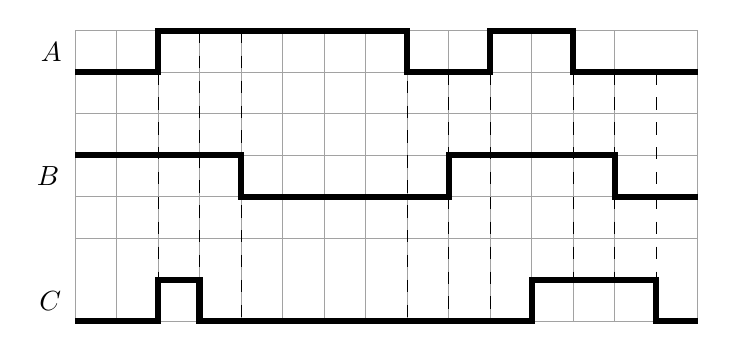
\begin{tikzpicture}[x=0.75pt,y=0.75pt,yscale=-1,xscale=1]
%uncomment if require: \path (0,300); %set diagram left start at 0, and has height of 300

%Shape: Grid [id:dp34531111101152123] 
\draw  [draw opacity=0] (100,40) -- (400,40) -- (400,180) -- (100,180) -- cycle ; \draw  [color={rgb, 255:red, 162; green, 162; blue, 162 }  ,draw opacity=1 ] (120,40) -- (120,180)(140,40) -- (140,180)(160,40) -- (160,180)(180,40) -- (180,180)(200,40) -- (200,180)(220,40) -- (220,180)(240,40) -- (240,180)(260,40) -- (260,180)(280,40) -- (280,180)(300,40) -- (300,180)(320,40) -- (320,180)(340,40) -- (340,180)(360,40) -- (360,180) ; \draw  [color={rgb, 255:red, 162; green, 162; blue, 162 }  ,draw opacity=1 ] (100,60) -- (400,60)(100,80) -- (400,80)(100,100) -- (400,100)(100,120) -- (400,120)(100,140) -- (400,140) ; \draw  [color={rgb, 255:red, 162; green, 162; blue, 162 }  ,draw opacity=1 ] (100,40) -- (400,40) -- (400,180) -- (100,180) -- cycle ;
%Straight Lines [id:da9908667716444586] 
\draw  [dash pattern={on 4.5pt off 4.5pt}]  (140,60) -- (140,160) ;


%Straight Lines [id:da9489034074703155] 
\draw  [dash pattern={on 4.5pt off 4.5pt}]  (160,40) -- (160,160) ;


%Straight Lines [id:da7444148673969375] 
\draw  [dash pattern={on 4.5pt off 4.5pt}]  (180,40) -- (180,180) ;


%Straight Lines [id:da33359589579811755] 
\draw  [dash pattern={on 4.5pt off 4.5pt}]  (260,40) -- (260,180) ;


%Straight Lines [id:da1689198722872045] 
\draw  [dash pattern={on 4.5pt off 4.5pt}]  (280,60) -- (280,180) ;


%Straight Lines [id:da2835936693187402] 
\draw  [dash pattern={on 4.5pt off 4.5pt}]  (300,60) -- (300,180) ;


%Straight Lines [id:da7069604701418795] 
\draw  [dash pattern={on 4.5pt off 4.5pt}]  (340,60) -- (340,160) ;


%Straight Lines [id:da35256438922338873] 
\draw  [dash pattern={on 4.5pt off 4.5pt}]  (360,60) -- (360,160) ;


%Straight Lines [id:da8396949759627998] 
\draw  [dash pattern={on 4.5pt off 4.5pt}]  (380,60) -- (380,160) ;


%Straight Lines [id:da8850959184881091] 
\draw [line width=2.25]    (100,60) -- (140,60) -- (140,40) -- (260,40) -- (260,60) -- (300,60) -- (300,40) -- (340,40) -- (340,60) -- (400,60) ;


%Straight Lines [id:da2574956876601695] 
\draw [line width=2.25]    (100,180) -- (140,180) -- (140,160) -- (160,160) -- (160,180) -- (320,180) -- (320,160) -- (380,160) -- (380,180) -- (400,180) ;


%Straight Lines [id:da8609754683162194] 
\draw [line width=2.25]    (100,100) -- (180,100) -- (180,120) -- (280,120) -- (280,100) -- (360,100) -- (360,120) -- (400,120) ;



% Text Node
\draw (88.5,50) node   {$A$};
% Text Node
\draw (87,110) node   {$B$};
% Text Node
\draw (88,170) node   {$C$};


\end{tikzpicture}
}

\end{frame}

\begin{frame}{Introdução}
\begin{block}{Derivada}
	\begin{itemize}
		\item A \textbf{derivada} de uma função $ f(t) $: as equações diferenciais utilizam as derivadas para descrever fenômenos físicos que variam com o tempo, onde o tempo varia \textbf{continuamente}.
	\end{itemize}

	\[ \od{f}{t}=\dot{f}=f^{\prime}=\lim\limits_{t\to t_0}\dfrac{f(t)-f(t_0)}{t-t_0} \]
	
\end{block}
\end{frame}

\begin{frame}{Introdução}
\begin{block}{Equação de diferenças}
	\begin{itemize}
		\item A \textbf{equação de diferenças} é qualquer problema onde deve-se determinar uma função desconhecida a partir de uma relação de recorrência envolvendo o operador diferença.
	\end{itemize}
	
	\[ \dfrac{\Delta f(t)}{\Delta t}=\dfrac{f(t)-f(t_0)}{t-t_0}\quad, \quad\forall (t-t_0) \in \set{\pm1, \pm2, \pm3, \ldots, \pm n} \subseteq \mathbb{Z}^{\times} \]
	
\end{block}
\end{frame}
	
\begin{frame}{Introdução}
\begin{block}{Equação de diferenças}
\begin{itemize}
	\item Os sinais de \textbf{entrada} passados após a $ k $-ésima amostra:  $ e_0$, $e_1$, $\ldots $, $ e_{k} $.
	\item Os sinais de \textbf{saída} anteriores a amostra $ k $: $ u_0$, $u_1$, $\ldots $, $ u_{k-1} $.
	\item Definimos a equação de recorrência $ u_k =f\left(e_0\ldots e_k, u_0\ldots u_{k-1} \right) $.
	\item De maneira geral: $$ \boxed{u(kT)=f\left[u(kT-T)\text{, }\ldots\text{, } u(kT-mT)\text{, }e(kT)\text{, }\ldots\text{, }e(kT-nT) \right]} $$
\end{itemize}

\textbf{Obs.:} É preciso de C.I.
\end{block}
\end{frame}

\begin{frame}{Exemplo \#01}
\begin{block}{Sequência de Fibonacci}
	\begin{minipage}{0.45\linewidth}
		\centering
		\[ u_k=u_{k-1}\mathord{+}\;u_{k-2}, \quad \text{onde }k\in \intco{2,\infty}\;\cap\;\mathbb{Z} \]
		
		\[ \begin{cases}
		u_0=1\\
		u_1=1
		\end{cases} \]
	\end{minipage}
	\hfill
	\begin{minipage}{0.45\linewidth}
		\centering
		\begin{longtable}{CC}
			\toprule
			k & u_k\\\midrule
			0 & 1\\
			1 & 1\\
			2 & 2\\
			3 & 3\\
			4 & 5\\
			5 & 8\\
			6 & 15\\
			7 & 21\\
			\multicolumn{2}{C}{\vdots} \\
			\bottomrule
		\end{longtable}
	\end{minipage}
\end{block}
\end{frame}

\begin{frame}{Exemplo \#01}
\begin{block}{Problema: determine $u_{50}$}
\begin{itemize}
    \item Preciso saber quem é $u_{49}$ e $u_{48}$.
    \item A \textbf{solução} consiste em encontrar uma forma de determinar $u(k)$ \textbf{independente} das amostras anteriores.
\end{itemize}
\end{block}
\end{frame}

\begin{frame}{Exemplo \#01}
\begin{block}{Solução}
No caso de Equações de Diferenças de Coeficientes Constantes (CCDE), a solução é no formato $z^k$, sendo $z$ a variável e $k$ a variável independente discreta.
\end{block}
\end{frame}

\begin{frame}{Exemplo \#01}
\begin{block}{Solução}
$$\boxed{u_k = Az^k}$$
A sequência de Fibonacci é dada por:
$$u_k = u_{k-1} + u_{k-2}$$
Com isso,
$$Az^k = Az^{k-1} + Az^{k-2}$$
$$Az^k = Az^k \cdot z^{-1} + Az^k \cdot z^{-2}$$
$$1 = z^{-1} + z^{-2}$$
Equação característica: $z^2 - z - 1 = 0 \implies z_{1,2} = \dfrac{1}{2} \pm \dfrac{\sqrt{5}}{2}$
\end{block}
\end{frame}

\begin{frame}{Exemplo \#01}
\begin{block}{Solução}
Considerando duas raízes reais, a solução geral é dada por:
$$u_k = A_1z_1^{k} + A_2z_2^{k}$$
Aplicando as condições iniciais, temos:
\begin{itemize}
    \item $u_0 = 1 \implies 1 = A_1z_1^{0} + A_2z_2^{0} \implies 1 = A_1 + A_2$
    \item $u_1 = 1 \implies 1 = A_1z_1^{1} + A_2z_2^{1} \implies 1 = A_1\left(\dfrac{1 + \sqrt{5}}{2}\right) + A_2\left(\dfrac{1 - \sqrt{5}}{2}\right)$
\end{itemize}
Multiplicando a primeira equação por $\left(\dfrac{1 + \sqrt{5}}{2}\right)$ e subtraindo da segunda, nos leva a:
$$A_2 = \dfrac{\sqrt{5} - 1}{2\sqrt{5}} \implies A_1 = \dfrac{\sqrt{5} + 1}{2\sqrt{5}}$$
\end{block}
\end{frame}

\begin{frame}{Exemplo \#01}
\begin{block}{Solução}
Com isso,
$$\boxed{u(k) = \dfrac{\sqrt{5} + 1}{2\sqrt{5}}\left(\dfrac{1 + \sqrt{5}}{2}\right)^k + \dfrac{\sqrt{5} - 1}{2\sqrt{5}}\left(\dfrac{1 - \sqrt{5}}{2}\right)^k}$$
\begin{itemize}
    \item \textbf{Independe} das amostras anteriores.
\end{itemize}
\end{block}
\end{frame}

\begin{frame}{Transformada $ \mathcal{Z} $}
\begin{block}{Definição}
	
\begin{minipage}{0.45\linewidth}
	\centering
	
	ED $ \rightarrow $ FT
	\[ \mathcal{L}\left\lbrace f(t) \right\rbrace=F(s) \]
	\[ s=\sigma+j\omega \]
\end{minipage}
\hfill
\begin{minipage}{0.45\linewidth}
	\centering
	
	ER $ \rightarrow $ FTD
	\[ \mathcal{Z}\left\lbrace f(kT) \right\rbrace=F(z) \]
	\[ z=\text{e}^{sT} \]
\end{minipage}

\vspace{0.5cm}

\textbf{Motivação}: estudo de filtros digitais, como implementar em um FPGA, por exemplo.

\end{block}
\end{frame}

\begin{frame}{Abordagem intuitiva (autofunções) - Exemplo \#01}
	\begin{center}
		\scalebox{1}{\deftkzbds
		
\begin{tikzpicture}[auto, node distance=2cm,>=Latex]
	% We start by placing the blocks
	\node [input] (input) {};
	\node [block, right=of input, xshift=0cm, align=center, text width=2cm] (computer) {$ h[n] $};
	\node [output, right =of computer] (output) {};
	\node [above, xshift=0.8cm] at (input) {$ x\left[n \right]  $};
	\node [above, xshift=-1cm] at (output) {$ y\left[n \right]  $};
	
	\draw [->] (input) -- (computer);
	\draw [->] (computer) -- (output);
\end{tikzpicture}}
	\end{center}
	
	\begin{block}{Problema}
		Dados: $ h[n]=\left( \dfrac{1}{2}\right)^{n}u[n]\, ,\quad \text{onde } u[n]=\begin{cases}
		1\, ,\, n\geqslant0.\\
		0\, ,\, n<0.
		\end{cases}  $
		
		\vspace{0.2cm}
		
		\textbf{Qual a resposta a $ \bm{x[n]=1} $?}
		
		\vspace{0.5cm}
		
		\textit{Dicas:}
		\begin{itemize}
			\item $ y[n]=x[n] * h[n]=\displaystyle\sum_{k=-\infty}^{\infty}h[k]x[n-k] $
			\item $ \displaystyle\sum_{k=0}^{\infty}r^{k}=\dfrac{1}{1-r}\, ,\, \text{se }|r|<1 $ (PG)
		\end{itemize}
	\end{block}
	
\end{frame}

\begin{frame}{Abordagem intuitiva (autofunções) - Exemplo \#01}
\begin{block}{Resolução}
	\[ y[n]=\sum_{k=-\infty}^{0}\cancelto{0}{\left( \dfrac{1}{2}\right)^{k}u[k]\cdot1}+\sum_{k=0}^{\infty}\left( \dfrac{1}{2}\right) ^{k}\cdot 1=\dfrac{1}{1-1/2}=\boxed{2} \]
\end{block}
\end{frame}

\begin{frame}{Abordagem intuitiva (autofunções) - Exemplo \#02}
\begin{center}
	\scalebox{1}{\deftkzbds
		
\begin{tikzpicture}[auto, node distance=2cm,>=Latex]
	% We start by placing the blocks
	\node [input] (input) {};
	\node [block, right=of input, xshift=0cm, align=center, text width=2cm] (computer) {$ h[n] $};
	\node [output, right =of computer] (output) {};
	\node [above, xshift=0.8cm] at (input) {$ x\left[n \right]  $};
	\node [above, xshift=-1cm] at (output) {$ y\left[n \right]  $};
	
	\draw [->] (input) -- (computer);
	\draw [->] (computer) -- (output);
\end{tikzpicture}}
\end{center}

\begin{block}{Problema}
	Dados: $ h[n]=\left( \dfrac{1}{2}\right)^{n}u[n]\, ,\quad \text{onde } u[n]=\begin{cases}
	1\, ,\, n\geqslant0\\
	0\, ,\, n<0
	\end{cases}  $
	
	\vspace{0.2cm}
	
	\textbf{E se $ \bm{x[n]=2^{n}} $?}
\end{block}
\end{frame}

\begin{frame}{Abordagem intuitiva (autofunções) - Exemplo \#02}
\begin{block}{Resolução}
	\begin{align*}
	y[n]&=\sum_{k=0}^{\infty}\left(\dfrac{1}{2} \right)^{k}\cdot2^{n-k}= \sum_{k=0}^{\infty}\left(\dfrac{1}{2} \right)^{k}\cdot2^{n}\cdot2^{-k}=\\
	&=2^{n}\sum_{k=0}^{\infty}\left(\dfrac{1}{2} \right)^{k}\cdot2^{-k}=2^{n}\sum_{k=0}^{\infty}\left(\dfrac{1}{2} \right)^{k}\cdot\left( \dfrac{1}{2}\right) ^{k}=\\
	&=2^{n}\sum_{k=0}^{\infty}\left(\dfrac{1}{4} \right)^{k}=2^{n}\cdot\dfrac{1}{1-1/4}=\boxed{\dfrac{4}{3}\cdot2^{n}}
	\end{align*}
\end{block}
\end{frame}

\begin{frame}{Abordagem intuitiva (autofunções) - Exemplo \#03}
\begin{center}
	\scalebox{1}{\deftkzbds
		
\begin{tikzpicture}[auto, node distance=2cm,>=Latex]
	% We start by placing the blocks
	\node [input] (input) {};
	\node [block, right=of input, xshift=0cm, align=center, text width=2cm] (computer) {$ h[n] $};
	\node [output, right =of computer] (output) {};
	\node [above, xshift=0.8cm] at (input) {$ x\left[n \right]  $};
	\node [above, xshift=-1cm] at (output) {$ y\left[n \right]  $};
	
	\draw [->] (input) -- (computer);
	\draw [->] (computer) -- (output);
\end{tikzpicture}}
\end{center}

\begin{block}{Problema}
	Dados: $ h[n]=\left( \dfrac{1}{2}\right)^{n}u[n]\, ,\quad \text{onde } u[n]=\begin{cases}
	1\, ,\, n\geqslant0\\
	0\, ,\, n<0
	\end{cases}  $
	
	\vspace{0.2cm}
	
	\textbf{De maneira geral: $ \bm{x[n]=z^{n}\, , \quad z} $ dado.}
\end{block}
\end{frame}

\begin{frame}{Abordagem intuitiva (autofunções) - Exemplo \#03}
\begin{block}{Resolução}
	\begin{align*}
	y[n]&=\sum_{k=0}^{\infty}\left(\dfrac{1}{2} \right)^{k}\cdot z^{n-k}=z^{n}\sum_{k=0}^{\infty}\left(\dfrac{1}{2} \right)^{k}\cdot z^{-k}\\
	&=z^{n}\sum_{k=0}^{\infty}\left(\dfrac{1}{2z} \right)^{k}=
	\left\{
	\begin{aligned}
	&\dfrac{1}{1-1/2z}\cdot z^{n}\tikzmark{af} &, \quad &\left| \dfrac{1}{2z} \right|<1\\
	&\infty &, \quad &\text{C.C.}
	\end{aligned}\right.
	\end{align*}
	
	\begin{tikzpicture}[overlay, remember picture]
	\draw[<-] (af) ++(0.2,0.5) -- +(1,0.5) node[above right=-6pt,yshift=-0.35cm,align=center, text width=2cm] {\textbf{autofunção} (analogia com autovetor)};
	\end{tikzpicture}
\end{block}
\end{frame}

\begin{frame}{Caso Geral}
\centering

\scalebox{1}{\deftkzbds

\begin{tikzpicture}[auto, node distance=2cm,>=Latex]
	% We start by placing the blocks
	\node [input] (input) {};
	\node [block, right=of input, xshift=0cm, align=center, text width=2cm] (computer) {$ h[n] $};
	\node [output, right =of computer] (output) {};
	\node [above, xshift=0.8cm] at (input) {$ z^{n} $};
	\node [above, xshift=-1cm] at (output) {$ H(z)z^{n} $};
	
	\draw [->] (input) -- (computer);
	\draw [->] (computer) -- (output);
\end{tikzpicture}}
\end{frame}

\begin{frame}{Caso Geral}
\begin{block}{Prova}
	\begin{align*}
	x[n]&=z^{n} \, , \quad z \text{ dado}\\
	y[n]&=x[n]*h[n]=\sum_{k=-\infty}^{\infty}h[k]x[n-k]=\sum_{k=-\infty}^{\infty}h[k]z^{n-k}=\\
	&=z^{n}\underbrace{\sum_{k=-\infty}^{\infty}h[k]z^{-k}}_{\substack{H(z) \\ \text{Transformada }\mathcal{Z}}}=H(z)z^{n}
	\end{align*}
	
	\QEDB
	
	\textbf{Obs.:} Note que o somatório \textbf{pode não convergir.}
\end{block}
	
\end{frame}


\begin{frame}{Região de convergência (ROC) - Exemplo \#01}
\begin{center}
	\scalebox{1}{\begin{tikzpicture}[scale=1.5,>=latex, every node/.style={inner sep=2pt}]
	
	\draw[pattern=south east lines, draw=mWhite] (0cm,0cm) circle(1.4cm);

	\draw[dashed] (0cm,0cm) circle(1.4cm);

	\draw[dashed, fill=mWhite] (0cm,0cm) circle(0.6cm);
	
    % draw the coordinates
    \draw[->, fill=mWhite] (-2cm,0cm) -- (2cm,0cm) node[right=2pt,fill=mWhite] {$\Re(z)$};
    \draw[->, fill=mWhite] (0cm,-2cm) -- (0cm,2cm) node[above=2pt,fill=mWhite] {$\Im(z)$};
    
    \draw[fill=black] (-1.4,0) ++(-2pt,-2pt) -- ++(4pt,4pt) ++(-4pt,0pt) -- ++(4pt,-4pt) +(-2pt,2pt) node[below left=2pt] {$ -1,4 $};
    
%    \draw[fill=black] (-0.6,0) circle (1pt) node[below=2pt,fill=mWhite] {$ -0,6 $};
    
    \draw[fill=black] (0.6,0) ++(-2pt,-2pt) -- ++(4pt,4pt) ++(-4pt,0pt) -- ++(4pt,-4pt) +(-2pt,2pt) node[below left=2pt] {$ 0,6 $};
    
%    \draw[fill=black] (1.4,0) circle (1pt) node[below=2pt,fill=mWhite] {$ 1,4$};

%	\draw[->] (0,0) -- (45:1) node[left] {$ r=1 $};
\end{tikzpicture}}
\end{center}

\begin{block}{Problema}
	$$ h[n]=\left( \dfrac{1}{2} \right)^{n}u[n] $$
	
	\textbf{Determine $ \bm{H(z)} $ e a sua ROC.}
\end{block}
\end{frame}


\begin{frame}{Região de convergência (ROC) - Exemplo \#01}
\begin{center}
	\scalebox{1}{\begin{tikzpicture}[scale=1.5,>=latex, every node/.style={inner sep=2pt}]
	
	\draw[pattern=south east lines, draw=mWhite] (0cm,0cm) circle(1.4cm);

	\draw[dashed] (0cm,0cm) circle(1.4cm);

	\draw[dashed, fill=mWhite] (0cm,0cm) circle(0.6cm);
	
    % draw the coordinates
    \draw[->, fill=mWhite] (-2cm,0cm) -- (2cm,0cm) node[right=2pt,fill=mWhite] {$\Re(z)$};
    \draw[->, fill=mWhite] (0cm,-2cm) -- (0cm,2cm) node[above=2pt,fill=mWhite] {$\Im(z)$};
    
    \draw[fill=black] (-1.4,0) ++(-2pt,-2pt) -- ++(4pt,4pt) ++(-4pt,0pt) -- ++(4pt,-4pt) +(-2pt,2pt) node[below left=2pt] {$ -1,4 $};
    
%    \draw[fill=black] (-0.6,0) circle (1pt) node[below=2pt,fill=mWhite] {$ -0,6 $};
    
    \draw[fill=black] (0.6,0) ++(-2pt,-2pt) -- ++(4pt,4pt) ++(-4pt,0pt) -- ++(4pt,-4pt) +(-2pt,2pt) node[below left=2pt] {$ 0,6 $};
    
%    \draw[fill=black] (1.4,0) circle (1pt) node[below=2pt,fill=mWhite] {$ 1,4$};

%	\draw[->] (0,0) -- (45:1) node[left] {$ r=1 $};
\end{tikzpicture}}
\end{center}

\begin{block}{Resolução}
	$$ h[n]=\left( \dfrac{1}{2} \right)^{n}u[n] $$
	
	\[ H(z)=\sum_{n=-\infty}^{\infty}h[n]z^{-n}=\sum_{n=0}^{\infty}\left( \dfrac{1}{2} \right)^{n}z^{-n}=\dfrac{1}{1-1/2z}\, , \, \left| \dfrac{1}{2z} \right|<1  \]
	
	\vspace{0.5cm}
	
	Logo, ROC: $ \set{z\in\mathbb{C}:|z|>1/2} $
	
\end{block}
\end{frame}


\begin{frame}{Região de convergência (ROC) - Exemplo \#02}
\begin{center}
	\scalebox{1}{\begin{tikzpicture}[scale=1.5,>=latex, every node/.style={inner sep=2pt}]
	
	\draw[pattern=south east lines, draw=mWhite] (0cm,0cm) circle(1.4cm);

	\draw[dashed] (0cm,0cm) circle(1.4cm);

	\draw[dashed, fill=mWhite] (0cm,0cm) circle(0.6cm);
	
    % draw the coordinates
    \draw[->, fill=mWhite] (-2cm,0cm) -- (2cm,0cm) node[right=2pt,fill=mWhite] {$\Re(z)$};
    \draw[->, fill=mWhite] (0cm,-2cm) -- (0cm,2cm) node[above=2pt,fill=mWhite] {$\Im(z)$};
    
    \draw[fill=black] (-1.4,0) ++(-2pt,-2pt) -- ++(4pt,4pt) ++(-4pt,0pt) -- ++(4pt,-4pt) +(-2pt,2pt) node[below left=2pt] {$ -1,4 $};
    
%    \draw[fill=black] (-0.6,0) circle (1pt) node[below=2pt,fill=mWhite] {$ -0,6 $};
    
    \draw[fill=black] (0.6,0) ++(-2pt,-2pt) -- ++(4pt,4pt) ++(-4pt,0pt) -- ++(4pt,-4pt) +(-2pt,2pt) node[below left=2pt] {$ 0,6 $};
    
%    \draw[fill=black] (1.4,0) circle (1pt) node[below=2pt,fill=mWhite] {$ 1,4$};

%	\draw[->] (0,0) -- (45:1) node[left] {$ r=1 $};
\end{tikzpicture}}
\end{center}

\begin{block}{Problema}
	$$ h[n]=-\left( \dfrac{1}{2}\right)^{n}u[-n-1] $$
	
	\textbf{Determine $ \bm{H(z)} $ e a sua ROC.}
\end{block}
\end{frame}


\begin{frame}{Região de convergência (ROC) - Exemplo \#02}
\begin{block}{Resolução}
	\[ u[-n-1]=0 \Rightarrow -n-1<0 \Rightarrow n>-1 \]
	\begin{align*}
	H(z)&=\sum_{n=-\infty}^{-1}-\left( \dfrac{1}{2}\right)^{n}z^{-n} \,\overset{k=-n}{\Longleftrightarrow}\, -\sum_{k=1}^{\infty}\left( \dfrac{1}{2}\right)^{-k}z^{k}=-\sum_{k=1}^{\infty}(2z)^{k}=
	\end{align*}
	\[ \boxed{\sum_{k=m}^{\infty}\dfrac{r^{m}}{1-r}} \]
	
	\[ =-2z\cdot\dfrac{1}{1-2z}\, , \, \left| 2z \right| < 1  \]
	
	\vspace{0.5cm}
	
	ROC: $ \set{z\in\mathbb{C} : |z| < 1/2} $
\end{block}
\end{frame}


\begin{frame}{Região de convergência (ROC)}
\begin{block}{Conclusão}
	
\begin{itemize}
	\item \textbf{Não dá para saber qual o sinal possui uma dada $ \bm{H(z)} $ sem saber a ROC.}
\end{itemize}

\vspace{0.5cm}

\begin{minipage}{0.4\linewidth}
	\begin{center}
		\scalebox{1}{\deftkzbds
	
\begin{tikzpicture}[auto, node distance=2cm,>=Latex]
	
	\node [input, name=input] {};
	\node [sum, right =of input, xshift=0.5cm] (sum) {$\sum$};
	\node [block, right =of sum, text width=2cm, align=center] (computer) {Computador digital};
	
	\node [block, right=of computer] (DA) {D/A};
	\draw [->] (computer) -- node[name=uk] {$u(kT)$} (DA);
	\node [block, right =of DA, pin={[pinstyle]above:$w(t)$},
	node distance=3cm] (process) {Planta};
	\node[below=20pt, circle, draw] at (process) {\Large 1};
	\draw [->] (DA) -- node[name=u] {$u(t)$} (process);
	% We draw an edge between the computer and process block to 
	% calculate the coordinate u. We need it to place the measurement block. 
	\node [output, right =of process] (output) {};
	
	\node [block, below=of computer, yshift=2cm, xshift=1.4em, minimum width=4em] (clock) {Clock};
	
	\node [block, below =of DA, pin={[pinstyle]below:$v(t)$}, yshift=-0.5cm] (sensor) {Sensor};
	\node [block, left=4cm] at (sensor) (AD) {A/D};
	\node[below=20pt, circle, draw] at (AD) {\Large 2};
	
	\draw [->] (clock) -| (DA);
	\draw [->] (clock) -| (AD);
	
	\draw [draw,->] (input) -- node {$r(kT)$} (sum);
	\draw [->] (sum) -- node {$\hat{e}(kT)$} (computer);
	\draw [->] (process) -- node [name=y] {$y(t)$}(output);
	\draw [->] (y) |- (sensor);
	\draw [->] (sensor) -- node[yshift=15pt] {$\hat{y}(t)$} (AD);
	\draw [->] (AD) -| node[pos=0.98, xshift=15pt] {$-$} node[pos=1.15, xshift=-4pt] {$+$} node [near start, yshift=15pt] {$\hat{y}(kT)$} (sum);
\end{tikzpicture}}
	\end{center}
\end{minipage}
\hfill
\begin{minipage}{0.55\linewidth}
	$$ \left\lbrace \begin{aligned}
	&z^{n}\sum_{n=-\infty}^{\infty}h[n]z^{-n} &, &\quad z\in \text{ROC}\\
	&\infty &, &\quad \text{C.C.}
	\end{aligned} \right.  $$
\end{minipage}
	
\end{block}
\end{frame}


\begin{frame}{ROC e estabilidade}
\begin{block}{}
	ROC: $ \set{z\in\mathbb{C} \text{ tal que } \displaystyle\sum_{n=-\infty}^{\infty}|h[n]z^{-n}|<\infty} $ \textbf{absolutamente somável}
	
	\begin{enumerate}
		\item Se $ z\in \text{ROC} \Rightarrow |H(z)|<\infty $
		\item Seja $ z $ na forma polar, $ z=r\text{e}^{j\omega} $, com $ r=|z| $, $ \omega=\phase{z} $
		\[ \Rightarrow \left| h[n]z^{-n} \right|=\left|h[n] \right|\cdot \left|z^{-n} \right|=|h[n]|\cdot r^{-n} \]
		$ \Rightarrow $ fato de $ z $ pertencer à ROC só depende de $ |z| $
	\end{enumerate}

\end{block}
\end{frame}


\begin{frame}{ROC e estabilidade}
\begin{block}{Condição de estabilidade}
	Para o sistema ser BIBO estável basta que a resposta ao impulso seja absolutamente somável.
	
	\[ |x[n]|\leqslant B\Rightarrow|y[n]|\leqslant C \]
\end{block}
\end{frame}

\begin{frame}{ROC e estabilidade}
\begin{block}{Condição de estabilidade}
	Prova:
	\begin{align*}
	y[n]&=\sum_{k=-\infty}^{\infty}h[k]x[n-k]\Rightarrow\\
	|y[n]|&=\left| \sum_{k=-\infty}^{\infty}h[k]x[n-k] \right| \quad \text{desigualdade de triângulos}\\
	|y[n]|&\leqslant \sum_{k=-\infty}^{\infty}\left|h[k]x[n-k] \right|
	\end{align*}
	
	
\end{block}
\end{frame}

\begin{frame}{ROC e estabilidade}
\begin{block}{Condição de estabilidade}
	\begin{align*}
	|y[n]|&\leqslant \sum_{k=-\infty}^{\infty}\left|h[k]\right| \cdot \left| x[n-k] \right|\\
	|y[n]|&\leqslant B \sum_{k=-\infty}^{\infty}\left|h[k]\right| \quad , \text{então}\\
	|y[n]|&\leqslant C
	\end{align*}
	\QEDB
	
\end{block}
\end{frame}

\begin{frame}{ROC e estabilidade}
\begin{block}{Condição de estabilidade}
	
	Portanto, o sistema é estável se $ \displaystyle\sum_{k=-\infty}^{\infty}|h[k]|<\infty $

\begin{itemize}
    \item \textbf{Exemplo:} a função degrau unitário é BIBO estável?
\end{itemize}

\end{block}
\end{frame}

\begin{frame}{ROC e estabilidade}
\begin{block}{Condição de estabilidade}
	Lembre-se que a condição de ROC é \[ \set{z\in\mathbb{C} \text{ tal que } \displaystyle\sum_{k=-\infty}^{\infty}|h[k]|\cdot r^{-k}<\infty}  \]
\end{block}
\end{frame}

\begin{frame}{ROC e estabilidade}
\begin{block}{Condição de estabilidade}
	Logo, o sistema é estável se e somente se $ r=1\in $ ROC.
\end{block}

\centering

\scalebox{1.5}{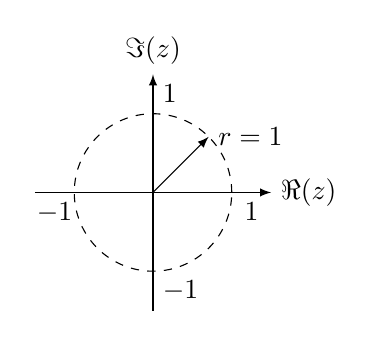
\begin{tikzpicture}[scale=1,>=latex]
        % draw the coordinates
        \draw[->] (-1.5cm,0cm) -- (1.5cm,0cm) node[right,fill=white] {$\Re(z)$};
        \draw[->] (0cm,-1.5cm) -- (0cm,1.5cm) node[above,fill=white] {$\Im(z)$};

        % draw the unit circle
        \draw[dashed] (0cm,0cm) circle(1cm);
        
        \draw[->] (0,0) -- (45:1) node[right] {$ r=1 $};

        % draw the horizontal and vertical coordinates
        % the placement is better this way
        \draw (-1.25cm,0cm) node[below] {$ -1 $}
              (1.25cm,0cm)  node[below] {$ 1 $}
              (0cm,-1.25cm) node[right] {$ -1 $}
              (0cm,1.25cm)  node[right] {$ 1 $};
    \end{tikzpicture}}

\end{frame}


\begin{frame}{ROC e causalidade}
\begin{block}{Sistemas causais}
	A saída \textbf{só depende da entrada no presente e no passado.} A saída não é antecipada antes da aplicação da entrada ($ h[n]=0\, , \, n<0 $).
	
	$$ y[n]=\sum_{k=0}^{\infty}h[k]x[n-k] \rightarrow y[n] \text{ só depende de } \left\lbrace \begin{aligned}&x[n] \quad &k=0\\
	&x[n-1] &k=1\\
	&x[n-2] &k=2\\
	& &\vdots\phantom{k=n}
	\end{aligned}\right.  $$
\end{block}
\end{frame}

\begin{frame}{ROC e causalidade}
\begin{block}{}
\begin{itemize}
	\item Para sistemas causais: $ h[n]=0 \, , \, n<0 $
\end{itemize}
\end{block}

\begin{minipage}{0.45\linewidth}
	\centering
	\scalebox{1}{\begin{tikzpicture}[y=0.75cm]
\draw[->] (-3,0) -- (1.5,0) node[right=2pt] {$ \sigma $};
\draw[->] (0,-4.5) -- (0,4.5) node[above=2pt] {$ j \omega $};

\draw[-{Latex[width=2pt, length=5pt]}] (-2,0) -- (-2,3.46);

\draw[dashed] (0,3.46) -- (-2,3.46);
\draw (-0.2,3.46) -- (0.2,3.46) node[right] {$ \num{3,46} $};

\draw[-{Latex[width=2pt, length=5pt]}] (0,0) -- (-2,3.46);
\draw (0,0) ++(-2pt,-2pt) -- ++(4pt,4pt) ++(-4pt,0pt) -- +(4pt,-4pt);

\draw (-0.2,-3.46) -- (0.2, -3.46) node[right] {$ \num{-3,46} $};

\draw[dashed] (-2,0) |- (0,-3.46);

\fill (-2,3.46) circle (1.2pt);

\node[below=2pt, fill=mWhite, inner sep=1pt] at (-2,0) {$ -2 $};

\draw[->] (0.5,0) arc (0:120:0.5cm) node[midway, above right=-3pt] {$ \gamma $};

\draw[->] (-1.7,0) arc (0:90:0.3cm) node[midway, above right=-3pt] {$ \alpha $};

\draw (-0.5,0) arc(180:120:0.5cm) node[left,midway] {$ \theta $};

\draw (-2,0) ++(-2pt,-2pt) -- ++(4pt,4pt) ++(-4pt,0pt) -- +(4pt,-4pt);

\end{tikzpicture}}
\end{minipage}
\hfill
\begin{minipage}{0.45\linewidth}
	\centering
	\[ h[n]=\left( \dfrac{1}{2} \right)^{n}u[n]  \]
	\[ \text{ROC: } |z|>1/2\]
	\scalebox{1}{\tikzset{every picture/.style={line width=0.75pt}} %set default line width to 0.75pt  

\begin{tikzpicture}[x=0.75pt,y=0.75pt,yscale=-1,xscale=1]

%uncomment if require: \path (0,300); %set diagram left start at 0, and has height of 300

%Straight Lines [id:da8305438567766523] 
\draw    (200.27,190.67) -- (365.77,190.67) ;
\draw [shift={(367.77,190.67)}, rotate = 180] [color={rgb, 255:red, 0; green, 0; blue, 0 }  ][line width=0.75]    (10.93,-3.29) .. controls (6.95,-1.4) and (3.31,-0.3) .. (0,0) .. controls (3.31,0.3) and (6.95,1.4) .. (10.93,3.29)   ;

%Shape: Circle [id:dp5343795865479193] 
\draw  [fill={rgb, 255:red, 255; green, 255; blue, 255 }  ,fill opacity=1 ] (207.97,191.08) .. controls (207.97,189.75) and (209.05,188.67) .. (210.38,188.67) .. controls (211.72,188.67) and (212.8,189.75) .. (212.8,191.08) .. controls (212.8,192.42) and (211.72,193.5) .. (210.38,193.5) .. controls (209.05,193.5) and (207.97,192.42) .. (207.97,191.08) -- cycle ;
%Shape: Circle [id:dp9958561748525927] 
\draw  [fill={rgb, 255:red, 255; green, 255; blue, 255 }  ,fill opacity=1 ] (227.57,190.68) .. controls (227.57,189.35) and (228.65,188.27) .. (229.98,188.27) .. controls (231.32,188.27) and (232.4,189.35) .. (232.4,190.68) .. controls (232.4,192.02) and (231.32,193.1) .. (229.98,193.1) .. controls (228.65,193.1) and (227.57,192.02) .. (227.57,190.68) -- cycle ;
%Straight Lines [id:da3574860753882376] 
\draw    (250.58,108.68) -- (250.58,190.28) ;


%Shape: Circle [id:dp04408180627185376] 
\draw  [fill={rgb, 255:red, 255; green, 255; blue, 255 }  ,fill opacity=1 ] (248.17,108.68) .. controls (248.17,107.35) and (249.25,106.27) .. (250.58,106.27) .. controls (251.92,106.27) and (253,107.35) .. (253,108.68) .. controls (253,110.02) and (251.92,111.1) .. (250.58,111.1) .. controls (249.25,111.1) and (248.17,110.02) .. (248.17,108.68) -- cycle ;
%Straight Lines [id:da7712579502140393] 
\draw    (270.58,129.5) -- (270.58,190.28) ;


%Shape: Circle [id:dp4215879501304003] 
\draw  [fill={rgb, 255:red, 255; green, 255; blue, 255 }  ,fill opacity=1 ] (268.17,129.5) .. controls (268.17,128.17) and (269.25,127.08) .. (270.58,127.08) .. controls (271.92,127.08) and (273,128.17) .. (273,129.5) .. controls (273,130.83) and (271.92,131.92) .. (270.58,131.92) .. controls (269.25,131.92) and (268.17,130.83) .. (268.17,129.5) -- cycle ;
%Straight Lines [id:da39800912811539835] 
\draw    (290.58,149.5) -- (290.58,190.28) ;


%Straight Lines [id:da15358320586768315] 
\draw    (311.08,171.5) -- (311.08,190.78) ;


%Shape: Circle [id:dp9326128099979845] 
\draw  [fill={rgb, 255:red, 255; green, 255; blue, 255 }  ,fill opacity=1 ] (288.17,149.5) .. controls (288.17,148.17) and (289.25,147.08) .. (290.58,147.08) .. controls (291.92,147.08) and (293,148.17) .. (293,149.5) .. controls (293,150.83) and (291.92,151.92) .. (290.58,151.92) .. controls (289.25,151.92) and (288.17,150.83) .. (288.17,149.5) -- cycle ;
%Shape: Circle [id:dp7866868035269907] 
\draw  [fill={rgb, 255:red, 255; green, 255; blue, 255 }  ,fill opacity=1 ] (308.67,169.08) .. controls (308.67,167.75) and (309.75,166.67) .. (311.08,166.67) .. controls (312.42,166.67) and (313.5,167.75) .. (313.5,169.08) .. controls (313.5,170.42) and (312.42,171.5) .. (311.08,171.5) .. controls (309.75,171.5) and (308.67,170.42) .. (308.67,169.08) -- cycle ;

% Text Node
\draw (334,178.5) node   {$\dotsc $};
% Text Node
\draw (371.5,200) node   {$n$};
% Text Node
\draw (251.5,200) node   {$0$};
% Text Node
\draw (271.5,200) node   {$1$};
% Text Node
\draw (292,200) node   {$2$};
% Text Node
\draw (312.5,200) node   {$3$};

\end{tikzpicture}}
\end{minipage}
\end{frame}


\begin{frame}{ROC e causalidade}
\begin{block}{}
	\begin{itemize}
		\item Para sistemas anticausais: $ h[n]=0 \, , \, n\geqslant0 $
	\end{itemize}
\end{block}
\begin{minipage}{0.45\linewidth}
	\centering
	\scalebox{1}{\begin{tikzpicture}
\draw (0,0) -- node[midway, below] {$ \dfrac{1}{T} $} (2.2,0);

\draw (0,0) -- (75:2.69);

\draw (0.3,0) arc (0:75:0.3) node[midway, right] {$ \ang{75} $};

\draw (2.2,0) -- +(120:3) node[midway,right] {$ \omega_n $};

\draw (1.9,0) arc (180:120:0.3) node[midway, left, yshift=2pt] {$ \theta $};

\draw (0.7,2.6) +(-0.13,-0.48) arc (255:300:0.5) node[coordinate, name=B] {};

\draw[->] (B) +(-0.2,0.1) parabola bend (1,2.4) (1.2,2.5) node[above] {$ \dfrac{\ang{180}-\theta}{2}-\dfrac{\phi}{2}=\ang{45} $};
\end{tikzpicture}}
\end{minipage}
\hfill
\begin{minipage}{0.45\linewidth}
	\centering
	\[ g[n]=-\left( \dfrac{1}{2} \right)^{n}u[-n-1]  \]
	\[ \text{ROC: } |z|<1/2\]
	\scalebox{1}{

\tikzset{every picture/.style={line width=0.75pt}} %set default line width to 0.75pt        

\begin{tikzpicture}[x=0.75pt,y=0.75pt,yscale=-1,xscale=1]
%uncomment if require: \path (0,300); %set diagram left start at 0, and has height of 300

%Straight Lines [id:da8305438567766523] 
\draw    (200.27,190.67) -- (365.77,190.67) ;
\draw [shift={(367.77,190.67)}, rotate = 180] [color={rgb, 255:red, 0; green, 0; blue, 0 }  ][line width=0.75]    (10.93,-3.29) .. controls (6.95,-1.4) and (3.31,-0.3) .. (0,0) .. controls (3.31,0.3) and (6.95,1.4) .. (10.93,3.29)   ;

%Shape: Circle [id:dp5343795865479193] 
\draw  [fill={rgb, 255:red, 255; green, 255; blue, 255 }  ,fill opacity=1 ] (347.47,190.58) .. controls (347.47,189.25) and (348.55,188.17) .. (349.88,188.17) .. controls (351.22,188.17) and (352.3,189.25) .. (352.3,190.58) .. controls (352.3,191.92) and (351.22,193) .. (349.88,193) .. controls (348.55,193) and (347.47,191.92) .. (347.47,190.58) -- cycle ;
%Shape: Circle [id:dp9958561748525927] 
\draw  [fill={rgb, 255:red, 255; green, 255; blue, 255 }  ,fill opacity=1 ] (328.07,190.68) .. controls (328.07,189.35) and (329.15,188.27) .. (330.48,188.27) .. controls (331.82,188.27) and (332.9,189.35) .. (332.9,190.68) .. controls (332.9,192.02) and (331.82,193.1) .. (330.48,193.1) .. controls (329.15,193.1) and (328.07,192.02) .. (328.07,190.68) -- cycle ;
%Straight Lines [id:da3574860753882376] 
\draw    (250.57,272.59) -- (250.57,191.28) ;


%Shape: Circle [id:dp04408180627185376] 
\draw  [fill={rgb, 255:red, 255; green, 255; blue, 255 }  ,fill opacity=1 ] (248.17,272.59) .. controls (248.17,273.92) and (249.24,275) .. (250.57,275) .. controls (251.9,275) and (252.98,273.92) .. (252.98,272.59) .. controls (252.98,271.26) and (251.9,270.18) .. (250.57,270.18) .. controls (249.24,270.18) and (248.17,271.26) .. (248.17,272.59) -- cycle ;
%Straight Lines [id:da7712579502140393] 
\draw    (270.5,251.85) -- (270.5,191.28) ;


%Shape: Circle [id:dp4215879501304003] 
\draw  [fill={rgb, 255:red, 255; green, 255; blue, 255 }  ,fill opacity=1 ] (268.1,251.85) .. controls (268.1,253.18) and (269.17,254.26) .. (270.5,254.26) .. controls (271.83,254.26) and (272.91,253.18) .. (272.91,251.85) .. controls (272.91,250.52) and (271.83,249.44) .. (270.5,249.44) .. controls (269.17,249.44) and (268.1,250.52) .. (268.1,251.85) -- cycle ;
%Straight Lines [id:da39800912811539835] 
\draw    (290.43,231.92) -- (290.43,191.28) ;


%Straight Lines [id:da15358320586768315] 
\draw    (310.86,210) -- (310.86,190.78) ;


%Shape: Circle [id:dp9326128099979845] 
\draw  [fill={rgb, 255:red, 255; green, 255; blue, 255 }  ,fill opacity=1 ] (288.02,231.92) .. controls (288.02,233.25) and (289.1,234.33) .. (290.43,234.33) .. controls (291.76,234.33) and (292.84,233.25) .. (292.84,231.92) .. controls (292.84,230.59) and (291.76,229.51) .. (290.43,229.51) .. controls (289.1,229.51) and (288.02,230.59) .. (288.02,231.92) -- cycle ;
%Shape: Circle [id:dp7866868035269907] 
\draw  [fill={rgb, 255:red, 255; green, 255; blue, 255 }  ,fill opacity=1 ] (308.45,212.41) .. controls (308.45,213.74) and (309.53,214.81) .. (310.86,214.81) .. controls (312.19,214.81) and (313.27,213.74) .. (313.27,212.41) .. controls (313.27,211.08) and (312.19,210) .. (310.86,210) .. controls (309.53,210) and (308.45,211.08) .. (308.45,212.41) -- cycle ;

% Text Node
\draw (224,203) node   {$\dotsc $};
% Text Node
\draw (371.5,197) node   {$n$};
% Text Node
\draw (310,180) node   {$-1$};
% Text Node
\draw (287,180) node   {$-2$};
% Text Node
\draw (265,180) node   {$-3$};
% Text Node
\draw (246,180) node   {$-4$};


\end{tikzpicture}
}
\end{minipage}

\end{frame}


\begin{frame}{ROC e polos}
\begin{block}{Contradição}
	\[ H(z)=\dfrac{N(z)}{D(z)} \]
	
	\[ \left. \begin{aligned}
	\text{Se } z \in \text{ ROC}&\Rightarrow |H(z)|<\infty\\
	\text{Se } z \text{ é polo} &\Rightarrow |H(z)|=\infty
	\end{aligned}\right\rbrace\, \bot  \]
	
	Logo, \textbf{polo $ \bm{\notin} $ ROC.}
\end{block}
\end{frame}


\begin{frame}{ROC e polos - Exemplo \#01}
	\begin{block}{Problema}
		\[ x[n]=\underbrace{\left( \dfrac{1}{2}\right)^{n}u[n]}_{h_1[n]}\underbrace{-2^{n}u[-n-1]\vphantom{\left(\dfrac{1}{2}\right)}}_{h_2[n]} \]
	\end{block}
\end{frame}


\begin{frame}{ROC e polos - Exemplo \#01}
\begin{block}{Resolução}
	\begin{align*}
		H_1(z)&=\dfrac{1}{1-1/2z}\, , \, |z|>\dfrac{1}{2}\\
		H_2(z)&=\dfrac{1}{1-2/z} \quad , \, |z|<2
	\end{align*}
\end{block}

\vspace{0.5cm}

\centering
\scalebox{0.8}{\deftkzbds

\begin{tikzpicture}[auto, node distance=1cm,>=Latex]
	% We start by placing the blocks
	\node [input] (input) {};
	\node [right=1cm, name=mid1, node distance=1pt, inner sep=1pt, fill=black, circle, draw] at (input) {};
	\node [right=1.3cm, name=mid] at (mid1) {};
	\node [block, above=0.5cm] at (mid) (h1) {$ h_1[n] $};
	\node [block, below=0.5cm] at (mid) (h2) {$ h_2[n] $};
	\node [sum, right=1cm, name=sum] at (mid) {$ + $};
	\node [output, right =of sum] (output) {};
	\node [above] at (input) {$ z^{n} $};
	\node [above] at (output) {$ y[n] $};
	
	\draw [->] (input) -| (mid1) |- (h1);
	\draw [->] (mid1) |- (h2);
	\draw [->] (h1) -| node[midway,right] {$ y_1[n] $} (sum);
	\draw [->] (h2) -| node[midway,right] {$ y_2[n] $} (sum);
	\draw [->] (sum) -- (output);
	
	\node[right=0.5cm, name=eq] at (output) {\Large $ \equiv $};
	
	\node [input, right=0.5cm] at (eq) (in2) {};
	\node [block, right=of in2] (computer) {$ x[n] $};
	\node [output, right =of computer] (out2) {};
	\node [above] at (in2) {$ z^{n} $};
	\node [above] at (out2) {$ y[n] $};
	
	\draw [->] (in2) -- (computer);
	\draw [->] (computer) -- (out2);
\end{tikzpicture}}

\end{frame}


\begin{frame}{ROC e polos - Exemplo \#01}
\begin{block}{Resolução}
	\centering
	\begin{align*}
	y_1[n]&=\left\lbrace \begin{aligned}
	&H_1(z)z^{n}& \, &, \, |z|>1/2\\
	&\infty& \, &, \, \text{C.C.}
	\end{aligned} \right.\\
	y_2[n]&=\left\lbrace \begin{aligned}
	&H_2(z)z^{n}& \, &, \, |z|<2\\
	&\infty& \, &, \, \text{C.C.}
	\end{aligned} \right.\\
	\Rightarrow y[n]& =\left\lbrace \begin{aligned}
	&z^{n}\left(H_1(z)+H_2(z) \right)& \, &, \, 1/2<|z|<2\\
	&\infty& \, &, \, \text{C.C.}
	\end{aligned} \right.
	\end{align*}
\end{block}
\end{frame}


\begin{frame}{ROC e polos - Exemplo \#01}
\begin{block}{Resolução}
	\[ X(z)=\dfrac{1}{1-1/2z}+\dfrac{1}{1-2/z}=\dfrac{2-\dfrac{5}{2}z^{-1}}{\left(1-\dfrac{1}{2}z^{-1} \right)\left(1-2z^{-1} \right)  } \]
	
	\begin{itemize}
		\item \textbf{Polos:} $ z=1/2 $ e $ z=2 $, ROC nunca atravessa o polo e é conexa.
		\item Sistema é \textbf{estável} ($ z=1 \in $ ROC).
	\end{itemize}
\end{block}
\end{frame}

\begin{frame}{Propriedades da ROC}
\begin{block}{Sinais de duração finita}
	A ROC de um sinal de duração finita inclui todo plano $z$, com possíveis exceções de $ z = 0 $ e $ |z| = \infty $.\\
	\begin{center}
		$ x[n] \neq 0 $, para $n_1 \leqslant n \leqslant n_2 $\\
		$$ X(z) = \sum_{n = n_1}^{n_2}x[n]z^{-n} $$
	\end{center}
	\begin{itemize}
		\item Se $ n_2 > 0 $: $ X(z) $ tem um termo $ z^{-1} $, logo a ROC não pode incluir $ z = 0 $.
		\item Se $ n_1 < 0 $: $ X(z) $ tem um termo $ z^{1} $, logo a ROC não pode incluir $ |z| = \infty $.
	\end{itemize}
\end{block}
\end{frame}

\begin{frame}{Propriedades da ROC}
\begin{block}{Sinais de duração finita - Exemplos}
	\begin{itemize}
		\item [1.] $ x[n] = \delta[n] $\\
		\vspace{0,1 cm}
		$ X(z) = \sum_{n=-\infty}^{\infty} \delta[n]z^{-n} = 1 $, \textbf{a ROC inclui todo plano $\bm{z}$!}\\
		\vspace{0,2 cm}
		\item [2.] $ x[n] = \delta[n - 1] $\\
		\vspace{0,1 cm}
		$ X(z) = \sum_{n=-\infty}^{\infty} \delta[n - 1]z^{-n} = z^{-1} = \dfrac{1}{z} $, a ROC não inclui $z=0$\\
		\vspace{0,2 cm}
		\item [3.] $ x[n] = \delta[n + 1] $\\
		\vspace{0,1 cm}
		$ X(z) = \sum_{n=-\infty}^{\infty} \delta[n + 1]z^{-n} = z $, a ROC não inclui $z = \infty$
	\end{itemize}
\end{block}
\end{frame}

\begin{frame}{Propriedades da ROC}
\begin{block}{Sinais de duração infinita - Resumo}
	A condição de convergência é $ |X(z)| < \infty $.
	\begin{itemize}
		\item A ROC de um sinal aberto à direita tem a forma $ |z| > r_{+} $.
		\item A ROC de um sinal aberto à esquerda tem a forma $ |z| <  r_{-} $.
		\item A ROC de um sinal bilateral tem a forma $ r_{+} < |z| < r_{-} $.
	\end{itemize}
\end{block}
\end{frame}

\begin{frame}{A relação entre a transformada $\mathcal{Z}$ e a transformada de Fourier}
\begin{block}{Transformada de Fourier para sinais discretos - \textit{DTFT}}
$$H(\text{e}^{j\omega}) = \sum_{n=-\infty}^{\infty}h[n]\text{e}^{-j\omega n}$$
\begin{itemize}
    \item $h[n]$ deve ser \textbf{absolutamente somável} para que o somatório convirja e, consequentemente, para que exista transformada de Fourier.
    \item Queremos ser capazes de representar com a transformada $\mathcal{Z}$ um sinal que \textbf{diverge}.
\end{itemize}
\end{block}
\end{frame}

\begin{frame}{A relação entre a transformada $\mathcal{Z}$ e a transformada de Fourier}
\begin{block}{Se $h[n]$ divergir...}
\begin{itemize}
    \item Podemos reescrever o sinal como:
\end{itemize}
$$\dfrac{h[n]}{r^n}$$
\begin{itemize}
    \item Para $|r| > 1$, $r^n$ também diverge.
    \item No entanto, se $r^n$ divergir \textbf{mais rapidamente} que $h[n]$, temos que o sinal, como um todo, \textbf{converge}. Desta forma, basta escolher um $r$ grande. 
\end{itemize}
\end{block}
\vspace{0.2cm}
\centering
\scalebox{0.8}{

\tikzset{every picture/.style={line width=0.75pt}} %set default line width to 0.75pt        

\begin{tikzpicture}[x=0.75pt,y=0.75pt,yscale=-1,xscale=1]
%uncomment if require: \path (0,300); %set diagram left start at 0, and has height of 300

%Straight Lines [id:da8305438567766523] 
\draw    (200.27,190.67) -- (365.77,190.67) ;
\draw [shift={(367.77,190.67)}, rotate = 180] [color={rgb, 255:red, 0; green, 0; blue, 0 }  ][line width=0.75]    (10.93,-3.29) .. controls (6.95,-1.4) and (3.31,-0.3) .. (0,0) .. controls (3.31,0.3) and (6.95,1.4) .. (10.93,3.29)   ;

%Shape: Circle [id:dp5343795865479193] 
\draw  [fill={rgb, 255:red, 255; green, 255; blue, 255 }  ,fill opacity=1 ] (347.47,190.58) .. controls (347.47,189.25) and (348.55,188.17) .. (349.88,188.17) .. controls (351.22,188.17) and (352.3,189.25) .. (352.3,190.58) .. controls (352.3,191.92) and (351.22,193) .. (349.88,193) .. controls (348.55,193) and (347.47,191.92) .. (347.47,190.58) -- cycle ;
%Shape: Circle [id:dp9958561748525927] 
\draw  [fill={rgb, 255:red, 255; green, 255; blue, 255 }  ,fill opacity=1 ] (328.07,190.68) .. controls (328.07,189.35) and (329.15,188.27) .. (330.48,188.27) .. controls (331.82,188.27) and (332.9,189.35) .. (332.9,190.68) .. controls (332.9,192.02) and (331.82,193.1) .. (330.48,193.1) .. controls (329.15,193.1) and (328.07,192.02) .. (328.07,190.68) -- cycle ;
%Straight Lines [id:da3574860753882376] 
\draw    (250.57,272.59) -- (250.57,191.28) ;


%Shape: Circle [id:dp04408180627185376] 
\draw  [fill={rgb, 255:red, 255; green, 255; blue, 255 }  ,fill opacity=1 ] (248.17,272.59) .. controls (248.17,273.92) and (249.24,275) .. (250.57,275) .. controls (251.9,275) and (252.98,273.92) .. (252.98,272.59) .. controls (252.98,271.26) and (251.9,270.18) .. (250.57,270.18) .. controls (249.24,270.18) and (248.17,271.26) .. (248.17,272.59) -- cycle ;
%Straight Lines [id:da7712579502140393] 
\draw    (270.5,251.85) -- (270.5,191.28) ;


%Shape: Circle [id:dp4215879501304003] 
\draw  [fill={rgb, 255:red, 255; green, 255; blue, 255 }  ,fill opacity=1 ] (268.1,251.85) .. controls (268.1,253.18) and (269.17,254.26) .. (270.5,254.26) .. controls (271.83,254.26) and (272.91,253.18) .. (272.91,251.85) .. controls (272.91,250.52) and (271.83,249.44) .. (270.5,249.44) .. controls (269.17,249.44) and (268.1,250.52) .. (268.1,251.85) -- cycle ;
%Straight Lines [id:da39800912811539835] 
\draw    (290.43,231.92) -- (290.43,191.28) ;


%Straight Lines [id:da15358320586768315] 
\draw    (310.86,210) -- (310.86,190.78) ;


%Shape: Circle [id:dp9326128099979845] 
\draw  [fill={rgb, 255:red, 255; green, 255; blue, 255 }  ,fill opacity=1 ] (288.02,231.92) .. controls (288.02,233.25) and (289.1,234.33) .. (290.43,234.33) .. controls (291.76,234.33) and (292.84,233.25) .. (292.84,231.92) .. controls (292.84,230.59) and (291.76,229.51) .. (290.43,229.51) .. controls (289.1,229.51) and (288.02,230.59) .. (288.02,231.92) -- cycle ;
%Shape: Circle [id:dp7866868035269907] 
\draw  [fill={rgb, 255:red, 255; green, 255; blue, 255 }  ,fill opacity=1 ] (308.45,212.41) .. controls (308.45,213.74) and (309.53,214.81) .. (310.86,214.81) .. controls (312.19,214.81) and (313.27,213.74) .. (313.27,212.41) .. controls (313.27,211.08) and (312.19,210) .. (310.86,210) .. controls (309.53,210) and (308.45,211.08) .. (308.45,212.41) -- cycle ;

% Text Node
\draw (224,203) node   {$\dotsc $};
% Text Node
\draw (371.5,197) node   {$n$};
% Text Node
\draw (310,180) node   {$-1$};
% Text Node
\draw (287,180) node   {$-2$};
% Text Node
\draw (265,180) node   {$-3$};
% Text Node
\draw (246,180) node   {$-4$};


\end{tikzpicture}
}
\end{frame}

\begin{frame}{A relação entre a transformada $\mathcal{Z}$ e a transformada de Fourier}
\begin{block}{Transformada $\mathcal{Z}$}
$$H(r,\text{e}^{j\omega}) = \sum_{n=-\infty}^{\infty}h[n]r^{-n} \text{e}^{-j\omega n}$$
$$H(r,\text{e}^{j\omega}) = \sum_{n=-\infty}^{\infty}h[n](r\text{e}^{j\omega})^{-n}$$
$$\boxed{H(z) = \sum_{n=-\infty}^{\infty}h[n]z^{-n}}$$
\begin{itemize}
    \item \textbf{Se \bm{$r = 1$}, a transformada \bm{$\mathcal{Z}$} coincide com a transformada de Fourier}.
\end{itemize}
\end{block}
\end{frame}

\begin{frame}{A relação entre a transformada $\mathcal{Z}$ e a transformada de Fourier}
\begin{block}{Exemplo \#01}
$$h[n] = \alpha^n u[n] \implies H(z) = \dfrac{1}{1 - \alpha z^{-1}}$$
$$\text{ROC: } |z|>|\alpha|$$
\begin{itemize}
    \item Se $|\alpha| > 1$ temos que $h[n]$ \textbf{diverge}.
    \begin{itemize}
        \item Se desenharmos a ROC, percebemos que não inclui a circunferência de raio unitário. Deste modo, este sinal \textbf{não tem} transformada de Fourier.
    \end{itemize}
    \item Se $|\alpha| < 1$ temos que $h[n]$ \textbf{converge}.
    \begin{itemize}
        \item Se desenharmos a ROC, percebemos que inclui a circunferência de raio unitário. Deste modo, este sinal \textbf{tem} transformada de Fourier.
    \end{itemize}
\end{itemize}
\end{block}
\end{frame}

\begin{frame}{A relação entre a transformada $\mathcal{Z}$ e a transformada de Fourier}
\begin{block}{Exemplo \#02}
$$h[n] = -\alpha^n u[-n-1] \implies H(z) = \dfrac{1}{1 - \alpha z^{-1}}$$
$$\text{ROC: } |z|<|\alpha|$$
\begin{itemize}
    \item Se $|\alpha| > 1$ temos que $h[n]$ \textbf{converge}.
    \begin{itemize}
        \item Se desenharmos a ROC, percebemos que inclui a circunferência de raio unitário. Deste modo, este sinal \textbf{tem} transformada de Fourier.
    \end{itemize}
    \item Se $|\alpha| < 1$ temos que $h[n]$ \textbf{diverge}.
    \begin{itemize}
        \item Se desenharmos a ROC, percebemos que não inclui a circunferência de raio unitário. Deste modo, este sinal \textbf{não tem} transformada de Fourier.
    \end{itemize}
\end{itemize}
\end{block}
\end{frame}

\begin{frame}{A relação entre a transformada $\mathcal{Z}$ e a transformada de Fourier}
\begin{block}{Problema}
	Determine a transformada $\mathcal{Z}$ do sinal\\
	$$ x[n] = \left\{\begin{matrix}
	1, & n = -1\\ 
	2, & n = 0\\ 
	-1, & n = 1\\ 
	1, & n = 2\\ 
	0, & \text{C.C.}
	\end{matrix}\right. $$\\
	Utilize a transformada $\mathcal{Z}$ para determinar a \textit{DTFT} de $x[n]$, caso exista.
\end{block}
\end{frame}

\begin{frame}{Propriedades da transformada $\mathcal{Z}$ bilateral}
\begin{block}{Propriedades}
	\begin{itemize}
		\item Reversão temporal
		$$ x[-n] \longleftrightarrow X\left( \dfrac{1}{z} \right), \quad \text{ ROC: } \dfrac{1}{R_x}$$
		\item Convolução
		$$ x[n]\ast y[n]  \longleftrightarrow X(z)Y(z), \quad \text{ ROC: } R_x \cap R_y $$
		\item Diferenciação no domínio z
		$$ nx[n] \longleftrightarrow -z\frac{\mathrm{d} }{\mathrm{d} x} X(z), \quad \text{ ROC: } R_x $$
	\end{itemize}
\end{block}
\end{frame}

\begin{frame}{Propriedades da transformada $\mathcal{Z}$ bilateral - Exemplo \#01}
\begin{block}{Problema}
		Encontre a transformada $\mathcal{Z}$ e a ROC do sinal\\
		$$ x[n] = \left ( n\left ( \dfrac{-1}{2} \right )^n u[n]\right )\ast\left ( \dfrac{1}{4} \right )^{-n}u[-n] $$
\end{block}
\end{frame}

\begin{frame}{Propriedades da transformada $\mathcal{Z}$ bilateral - Exemplo \#01}
\begin{block}{Resolução}
	$$ x[n] = \underset{x_1[n]}{\underbrace{\left ( n\left ( \dfrac{-1}{2} \right )^n u[n]\right )}}\ast \underset{x_2[n]}{\underbrace{\left ( \dfrac{1}{4} \right )^{-n}u[-n]}} $$
	\begin{itemize}
	    \item Aplicando as propriedades, temos:
	\end{itemize}
	$$ X_1(z) = \dfrac{-\frac{1}{2}z}{\left ( z + \frac{1}{2} \right )^2}, \quad \text{ ROC: } \left | z \right |  > \frac{1}{2} $$
	$$ X_2(z) = \dfrac{-4}{z - 4}, \quad \text{ ROC: } \left | z \right |  < 4 $$
	\vspace{-0.2cm}
	\begin{itemize}
	    \item Deste modo,
	\end{itemize}
	$$ X(z) = \dfrac{2z}{\left ( z + \frac{1}{2} \right )^2 (z - 4)}, \quad \text{ ROC: } \frac{1}{2}< \left | z \right |  < 4 $$
\end{block}
\end{frame}

\begin{frame}{Propriedades da transformada $\mathcal{Z}$ unilateral}
\begin{block}{Linearidade}
A transformada $\mathcal{Z}$ é uma transformada \textbf{linear}. Considere um sinal $x[n]$ cuja transformada $\mathcal{Z}$ é $X(z)$, e considere ainda um sinal $y[n]$ cuja transformada $\mathcal{Z}$ é $Y(z)$. Deste modo:

$$\mathcal{Z}\{\alpha x[n] + \beta y[n]\} = \alpha X(z) + \beta Y(z)$$ \\
\vspace{0.2cm}
\textbf{Demonstração}: 
$$\mathcal{Z}\{\alpha x[n] + \beta y[n]\} = \sum_{n=0}^{\infty} \left[\alpha x[n] + \beta y[n]\right] z^{-n}$$
$$= \alpha \sum_{n=0}^{\infty} x[n] z^{-n} + \beta \sum_{n=0}^{\infty} y[n] z^{-n} = \alpha X(z) + \beta Y(z)$$ \qed
\end{block}
\end{frame}

\begin{frame}{Propriedades da transformada $\mathcal{Z}$ unilateral}
\begin{block}{Deslocamento no tempo (atraso)}
Se $\mathcal{Z}\{x[n]\} = X(z)$ então $\mathcal{Z}\{x[n-n_0]\} = z^{-n_0} \left(X(z) + \sum_{\gamma=1}^{n_0} x[-\gamma] z^{\gamma}  \right)$ \\
\vspace{0.2cm}
\textbf{Demonstração}: Seja $n - n_0 = \gamma$, então:
$$\mathcal{Z}\{x[n-n_0]\} = \sum_{n=0}^{\infty} x[n-n_0] z^{-n} = \sum_{\gamma=-n_0}^{\infty} x[\gamma] z^{-(\gamma + n_0)} = z^{-n_0} \sum_{\gamma=-n_0}^{\infty} x[\gamma] z^{-\gamma}$$
$$= z^{-n_0} \sum_{\gamma=-n_0}^{\infty} x[\gamma] z^{-\gamma} - z^{-n_0} \sum_{\gamma=-n_0}^{-1} x[\gamma] z^{-\gamma} + z^{-n_0} \sum_{\gamma=-n_0}^{-1} x[\gamma] z^{-\gamma}$$
$$= z^{-n_0} \sum_{\gamma=0}^{\infty} x[\gamma] z^{-\gamma} + z^{-n_0} \sum_{\gamma=-n_0}^{-1} x[\gamma] z^{-\gamma} = z^{-n_0} \left(X(z) + \sum_{\gamma=1}^{n_0} x[-\gamma] z^{\gamma}\right)$$\qed
\end{block}
\end{frame}

\begin{frame}{Propriedades da transformada $\mathcal{Z}$ unilateral}
\begin{block}{Deslocamento no tempo (avanço)}
Se $\mathcal{Z}\{x[n]\} = X(z)$ então $\mathcal{Z}\{x[n+n_0]\} = z^{n_0} \left(X(z) - \sum_{\gamma=0}^{n_0-1} x[\gamma] z^{-\gamma}  \right)$ \\
\vspace{0.2cm}
\textbf{Demonstração}: Seja $n + n_0 = \gamma$, então:
$$\mathcal{Z}\{x[n+n_0]\} = \sum_{n=0}^{\infty} x[n+n_0] z^{-n} = \sum_{\gamma=n_0}^{\infty} x[\gamma] z^{-(\gamma - n_0)} = z^{n_0} \sum_{\gamma=n_0}^{\infty} x[\gamma] z^{-\gamma}$$
$$= z^{n_0} \sum_{\gamma=n_0}^{\infty} x[\gamma] z^{-\gamma} + z^{n_0} \sum_{\gamma=0}^{n_0-1} x[\gamma] z^{-\gamma} - z^{n_0} \sum_{\gamma=0}^{n_0-1} x[\gamma] z^{-\gamma}$$
$$= z^{n_0} \sum_{\gamma=0}^{\infty} x[\gamma] z^{-\gamma} - z^{n_0} \sum_{\gamma=0}^{n_0-1} x[\gamma] z^{-\gamma} = z^{n_0} \left(X(z) - \sum_{\gamma=0}^{n_0-1} x[\gamma] z^{-\gamma}\right)$$\qed
\end{block}
\end{frame}


\frame{
\frametitle{Exercícios}
\begin{block}{}
01. Demonstre a propriedade do deslocamento no tempo (atraso) para a transformada $\mathcal{Z}$ bilateral. Qual a diferença quando comparada com a transformada $\mathcal{Z}$ unilateral?

\vspace{1cm}

02. Demonstre a propriedade do deslocamento no tempo (avanço) para a transformada $\mathcal{Z}$ bilateral. Qual a diferença quando comparada com a transformada $\mathcal{Z}$ unilateral?
\end{block}
}

\frame{
\frametitle{Exercícios}
\begin{block}{}
03. A acumulação no domínio do tempo discreto é análoga à integração no domínio do tempo contínuo. Considere a acumulação
$$y[n] = \sum_{k=-\infty}^{n} x[n]$$
Mostre que a transformada $\mathcal{Z}$ (independente se bilateral ou unilateral) é dada por
$$\dfrac{Y(z)}{X(z)} = \dfrac{z}{z-1}$$
\end{block}
}

\frame{
\frametitle{Referências e exercícios complementares}
\begin{itemize}
\item AGUIRRE, Luis A. Controle de Sistemas Amostrados, 1 ed. [s.n.], 2019.
\end{itemize}
\centering{\alert{Página 96 - \textbf{Capítulo 3}}} \\
\vspace{0.4cm}
\begin{itemize}
\item FRANKLIN, Gene F.; POWELL, J. David; WOLKMAN, Michael L. Digital Control of Dynamic Systems, 3 ed. Addison-Wesley, 1998.
\end{itemize}
\centering{\alert{Página 149 - \textbf{Capítulo 4}}} \\
}
